\documentclass[border=10pt]{standalone}

\usepackage{tikz}
\usepackage{tikzsymbols}
\usetikzlibrary{calc,patterns,shapes.geometric}

\def\centerarc[#1](#2)(#3:#4:#5){\draw[#1] ($(#2)+({#5*cos(#3)},{#5*sin(#3)})$) arc (#3:#4:#5);}

\begin{document}
	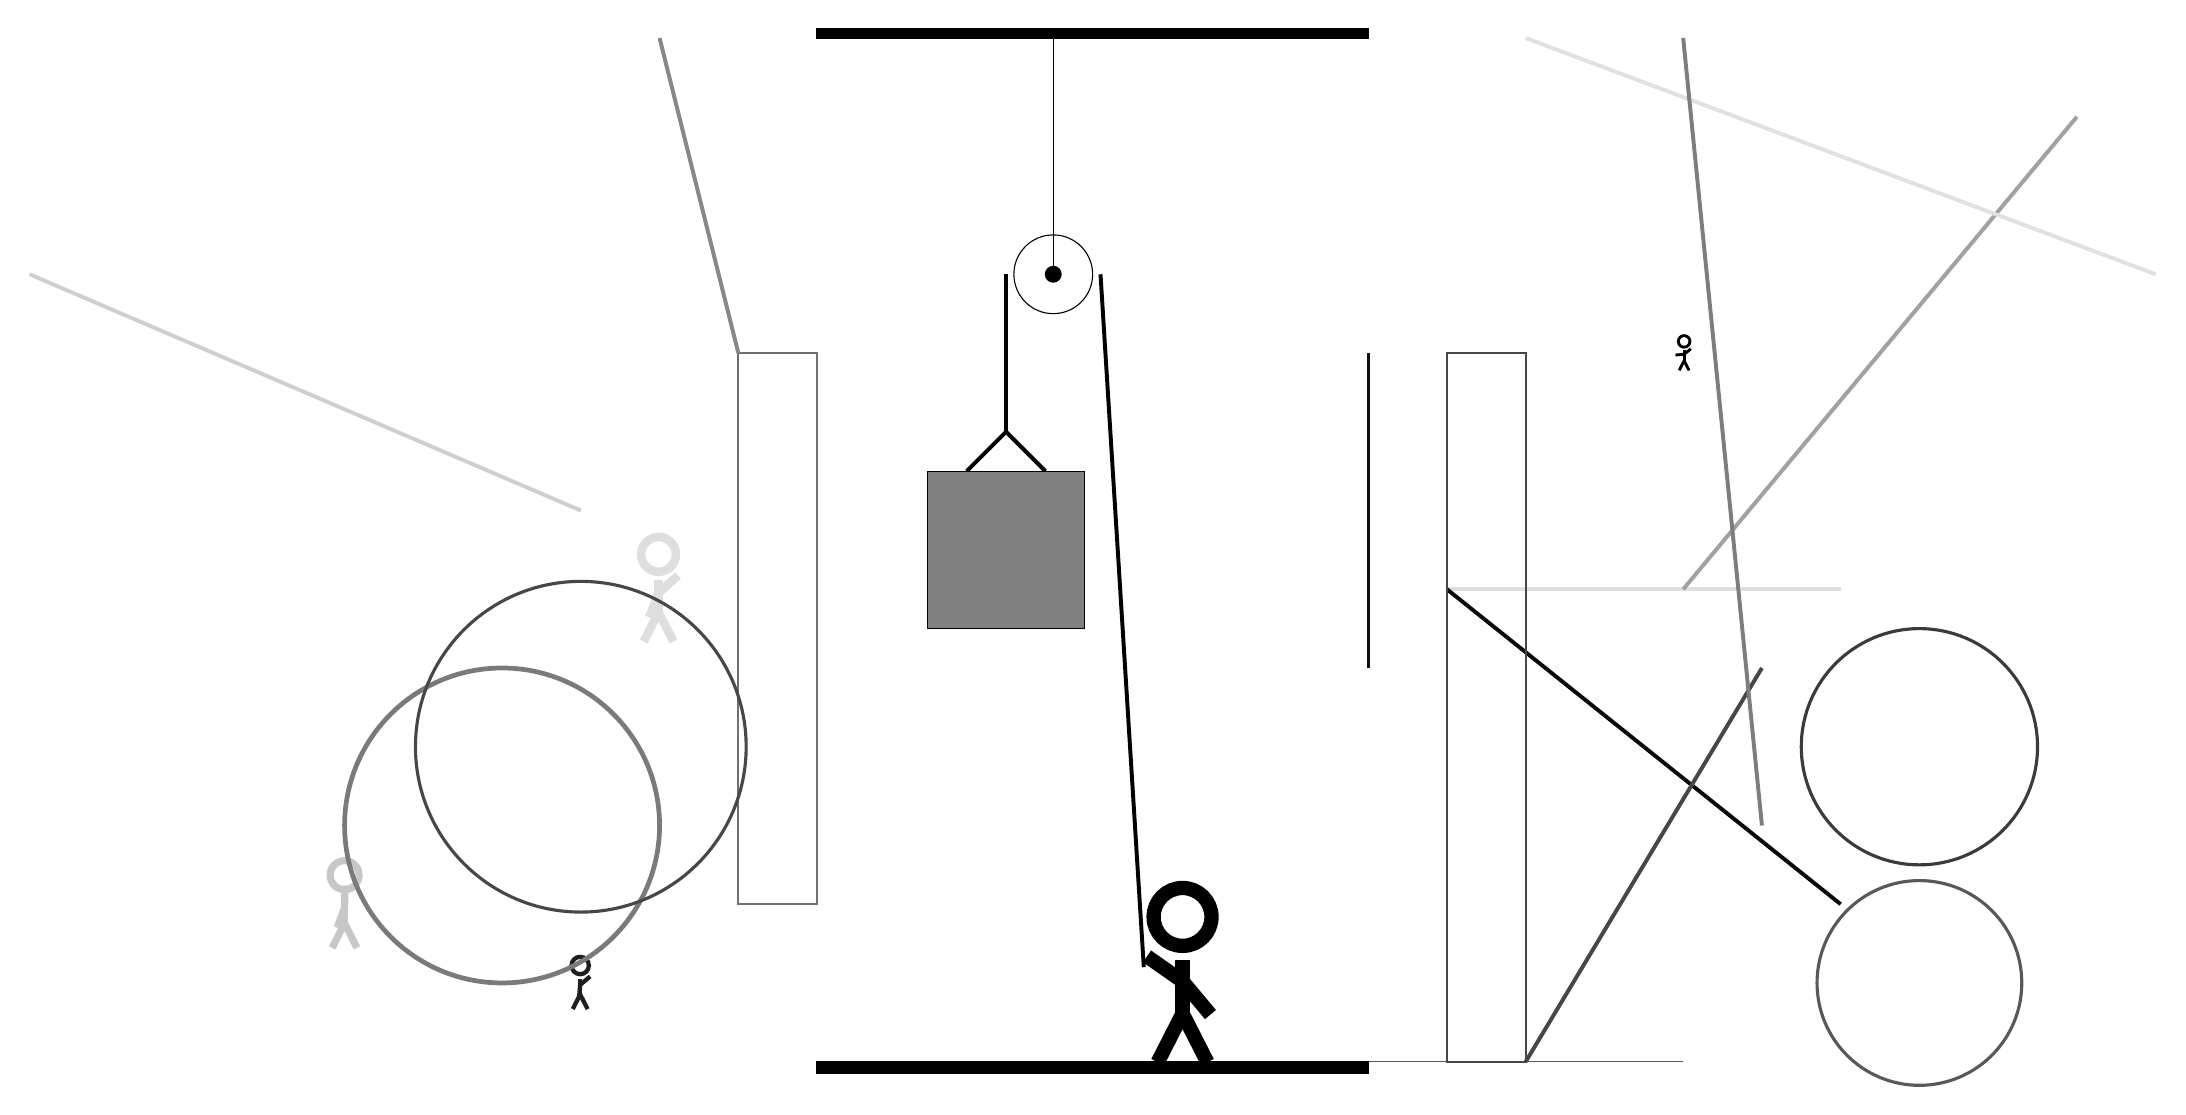
\begin{tikzpicture}
		%%%%% START %%%%%
		
		\draw[fill=black] (-2, 10) rectangle (5, 10.125);
		
		\draw (1, 7) circle (0.5);
		\draw[fill=black] (1, 7) circle (0.1);
		\draw (1, 10) -- (1, 7);
		
		\draw[line width=0.5mm] (-0.1, 4.5) -- (0.4, 5.0) -- (0.9, 4.5);
		\draw[fill=black!50] (-0.6, 4.5) rectangle (1.4, 2.5);
		
		\draw[line width=0.5mm] (0.4, 7) -- (0.4, 5.0);
		\centerarc[line width=0.5mm](1, 7)(0:180:0.6);
		\draw[line width=0.5mm](1.6, 7) -- (2.15, -1.8);
		
		\draw[line width=0.5mm, color=black!13](6, 3) -- (11, 3);
		
		\draw[line width=0.5mm, color=black!96](6, 3) -- (11, -1);
		\draw[line width=0.2mm, color=black!65] (5, -3) rectangle (9, -3);
		\draw[line width=0.3mm, color=black!72] (6, -3) rectangle (7, 6);
		\draw[line width=0.5mm, color=black!37](9, 3) -- (14, 9);
		\node[line width=0.4mm, color=black!22] at (-8, -1) {\Strichmaxerl[5][70][89]};
		\node[line width=0.3mm, color=black!88] at (-5, -2) {\Strichmaxerl[3][85][40]};
		\draw[line width=0.5mm, color=black!12](7, 10) -- (15, 7);
		\draw [line width=0.4mm, color=black!65](12, -2) circle (1.3);
		
		\draw [line width=0.4mm, color=black!77](12, 1) circle (1.5);
		\node[line width=0.7mm, color=black!13] at (-4, 3) {\Strichmaxerl[6][69][42]};
		
		\draw[line width=0.3mm, color=black!56] (-2, 6) rectangle (-3, -1);
		\node[line width=0.3mm, color=black!100] at (9, 6) {\Strichmaxerl[2][5][39]};
		
		\draw[line width=0.4mm, color=black!94] (5, 6) rectangle (5, 2);
		\draw [line width=0.6mm, color=black!52](-6, 0) circle (2.0);
		\draw[line width=0.5mm, color=black!72](10, 2) -- (7, -3);
		
		\draw[line width=0.5mm, color=black!19](-5, 4) -- (-12, 7);
		\draw [line width=0.4mm, color=black!72](-5, 1) circle (2.1);
		\draw[line width=0.5mm, color=black!51](9, 10) -- (10, 0);
		\draw[line width=0.5mm, color=black!47](-3, 6) -- (-4, 10);
		
		\node at (2.6, -1.9) {\Strichmaxerl[10][-35][-50]};
		
		\draw[fill=black] (-2, -3) rectangle (5, -3.15);
		
		%%%%% END %%%%%
	\end{tikzpicture}
\end{document}